\subsection{Analyse}
Der er udarbejdet en række diagrammer over de to detaljerede brugsmønstre.\\
Der er to forskellige typer af analysediagrammer, der er de dynamiske og de statisk.

\subsubsection{Statiske side af analysen}
Der er udarbejdet et klassediagram (Se figur \ref{fig:AKlasse}) som består af 9 klasser: Afdeling, Sag, Afgørelsesbrev, Ydelse, Person, Sekretær, Sagsbehandler, Afdelingsleder og Borger. De to mest centrale klasser i diagrammet er Afdeling og Sag, som skaber grundlaget for systemet. \\ 
\begin{figure}[h]
  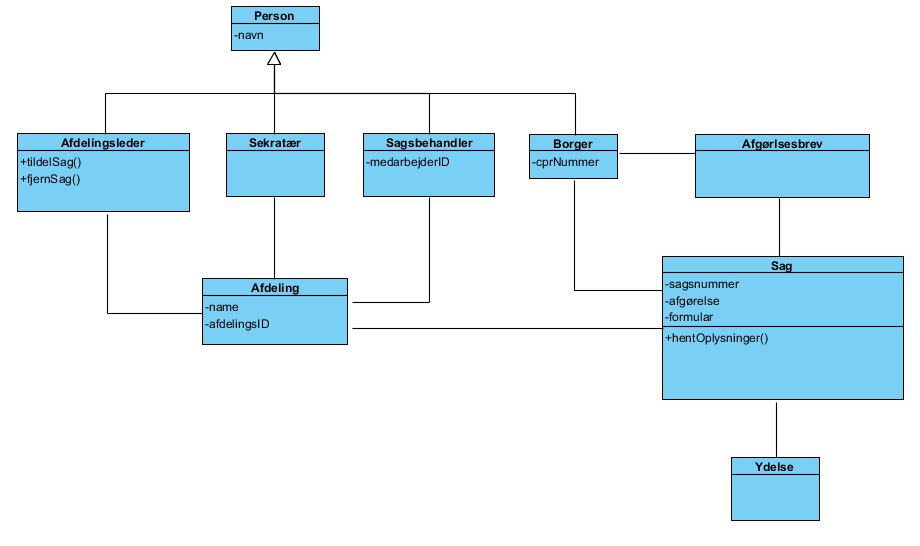
\includegraphics[width=\linewidth]{./PNG/analyse/analyseKlasseDiagram.PNG} 
  \caption{Analyseklassediagram. For fuld størrelse se interne bilag afsnit \ref{sec:diverse} figur \ref{fig:fuldDesignKlasseDiagram}}
  \label{fig:AKlasse}
\end{figure}
\\Afdeling består af attributterne ”navn” og ”afdelingsID”, som blev valgt for at muliggøre identifikationen af en afdeling. Klassen er central for systemet da den skal bruges til at administrere dem som arbejder i en afdeling og hvilke sager de er ansvarlige for. \\ 
\\
Sag er en klasse, som består af attributterne ”sagsnummer”, ”afgørelse” og ”formular”, samt metoden ”hentOplysninger()”. Klassen udgør omdrejningspunktet i arbejdet med sagsbehandling, da Sag klassen skal bruges i forbindelse med behandling af borgere. Attributten ”formular”, repræsentere de dokumenter der, ifølge VUM, (Anon., 2019) skal udfyldes af personalet f.eks. sagsbehandler. \\ 
\\
Sag er forbundet til Afdeling for at indikere at en sag behandles i en specifik afdeling.\\
Ydelse er en klasse som repræsenterer hvilke botilbud og lignende som tildeles en borger ud fra deres behov. Ydelse er forbundet til Sag, da den tildeles baseret på en vurdering af en specifik sag. En borger kan modtage flere ydelser, men disse ydelser er alle baseret på de specifikke sager som berør den enkelte borger.\\ 
\\
Borger klassen repræsenterer en person som skal registreres i systemet for at modtage et givent tilbud. Borger klassen har attributten ”cpr-nummer”, som bruges til at identificere den borgeren. Yderligere arver Borger klassen fra Person, som giver attributten ”navn”.
\subsubsection{Dynamiske side af analysen}
\begin{figure}[htb!]
  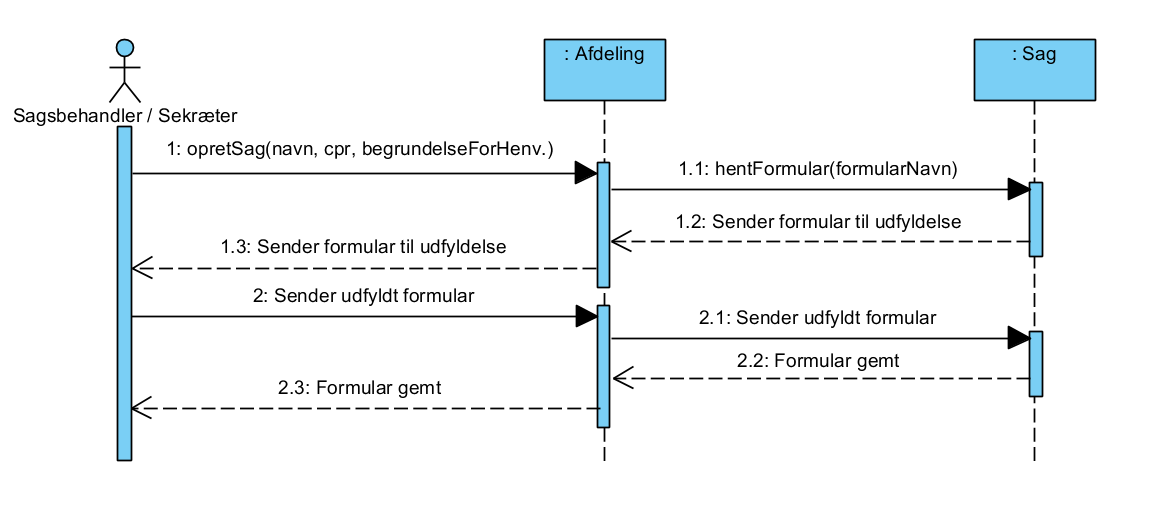
\includegraphics[width=\linewidth]{./PNG/analyse/opretSag.PNG} 
  \caption{Sekvensdiagram for opret sag}
  \label{fig:opretSag}
\end{figure}
\textbf{Opret sag}\\
Beskrivelse:\\
Som man kan se på figur \ref{fig:opretSag} påbegynder operationen opretSag ved at en af aktøren, sagsbehandler eller sekretær anmoder systemet om at oprette en sag til afdeling. Afdelingen håndterer operationen ved at hente en formular ved at sende forespørgsel til Sag objektet. Objektet tilbagesender en pågældende formular tilbage til afdeling objektet. Når afdelingen modtager formularen, videresendes den til den pågældende aktør. Aktøren udfylder formularen med relevante oplysninger, hvorefter den sendes til afdelingen, hvor denne sender det videre til den pågældende sag for opdatering. \\ \\
Evaluering:\\
Det er vigtigt for en sagsbehandler eller sekretær at kunne oprette en sag på en boger. Operationen opretSag er er starten for selve sagsforløbet og dermed essentiel del for systemet. \\
\begin{figure}[htb!]
  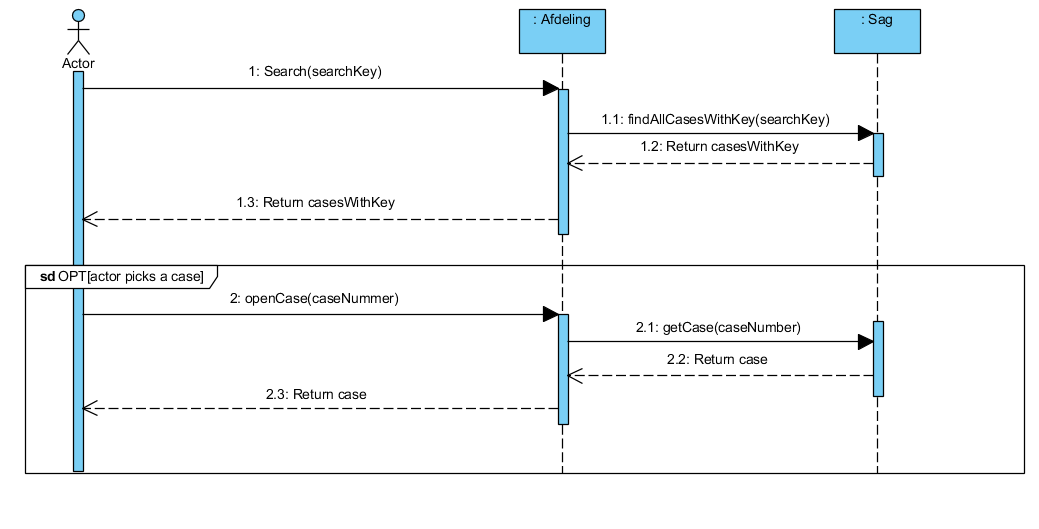
\includegraphics[width=\linewidth]{./PNG/analyse/findSag.PNG} 
  \caption{Sekvensdiagram for find sag}
  \label{fig:findSag}
\end{figure}\\
\textbf{Find sag}\\
Beskrivelse: \\
En aktør, f.eks. sagsbehandler eller sekretær, vælger at søge på en sag, som vist i figur \ref{fig:findSag}. Search metoden modtager en nøgle værdi. Den sender besked ned til afdelingen og herefter spørger en metode efter at finde alle sager med den specifikke nøgleværdi. Sager med den specifikke nøgle sendes tilbage til afdelingen og afdelingen sender resultatet videre til aktøren. Herefter vælger aktøren at åbne den specifikke sag, hvor der kaldes på openCase metoden som sender besked ned til afdelingen. Afdelingen efterspørger herefter om at få den sag med det specifikke sagsnummer, og der returneres et sagsobjekt med det specifikke sagsnummer. Afdelinger returner efterfølgende det fundne sagsobjekt til aktøren. \\ \\
Vurdering:\\
Det er vigtigt for en sagsbehandler eller en sekretær at kunne finde sager vedrørende en borger. Dermed når en borger henvender sig, kan en sekretær søge en sag frem på den pågældende borger.  
